\section{Single Operation Experiments}
We have attempted to experimentally determine the running times, or rather, the difference in running time of our implementations of \verb#Insert#, \verb#DeleteMin# and \verb#DecreaseKey# in the two types of heaps. We have done so by running each operation 5, 10, 15, 20, 25, 30 and 35 million times on each type of heap. We have also counted the number of comparisons done by each heap for the operations.

\subsection{Running Times}
We have measured the running time using the difference of two calls to \verb#clock()#, one right before and one right after the experiment, converting into seconds by division with CLOCKS\_PER\_SEC.

\subsubsection{Insert}
Testing the running time of the insert operation was done by inserting elements with integer keys between $0$ and $n-1$ in reverse order, so that each element inserted had the lowest key, to simulate a worst-case situation where each newly inserted element is the new minimum.

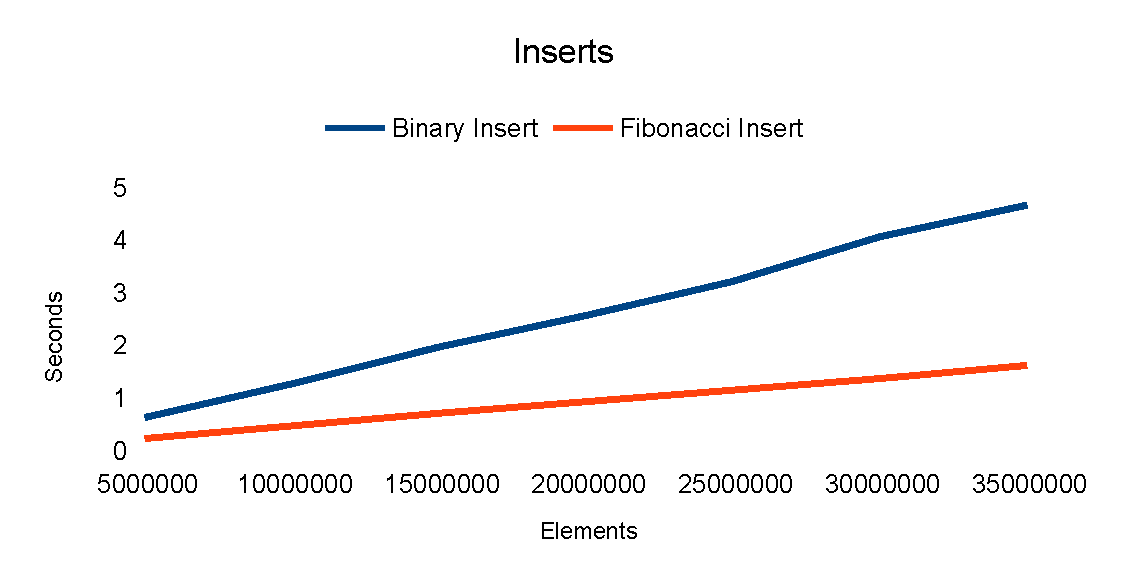
\includegraphics[width=\textwidth]{graphs/insert_graph.pdf}

We can see that the fibonacci heap is considerably faster for this operation.

\subsubsection{DeleteMin}
Testing the running time of the deletemin operation consisted of first inserting the relevant amount of elements exactly like in the test of inserts, then resetting the comparison count, and then running DeleteMin on the heap an equal amount of times only running the clock while the deletemin operations were running.

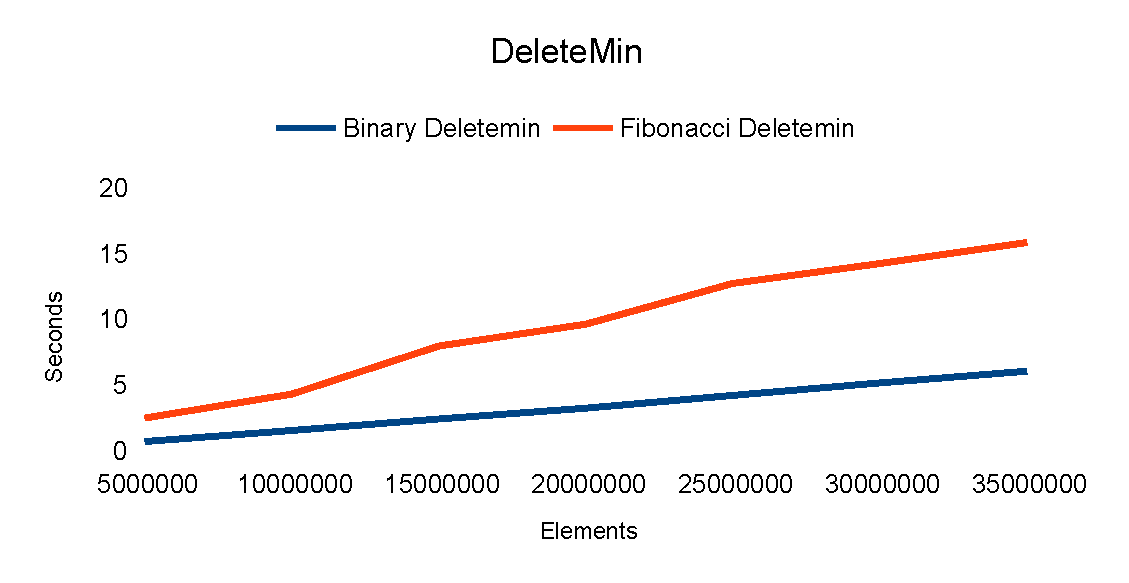
\includegraphics[width=\textwidth]{graphs/deletemin_graph.pdf}

We can see that, for this operation, the binary heap is the faster one.

\subsubsection{DecreaseKey}
The setup for this test was the same as for DeleteMin. The test itself consisted of going through each inserted element, decreasing its key to a new minimum (one below the previous minimum). This was repeated 5 times.

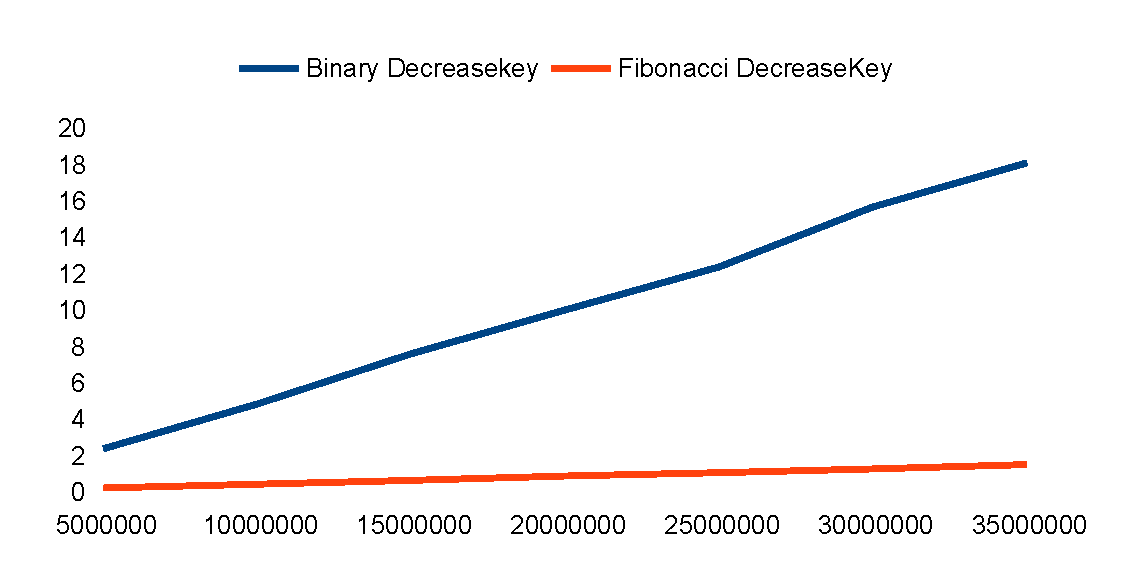
\includegraphics[width=\textwidth]{graphs/decreasekey_graph.pdf}

For this operation, we again see the fibonacci heap being much faster.

\subsection{Comparisons}
Counting the comparisons was done simply by keeping a counter variable in the heap and upcounting it whenever a comparison was done.

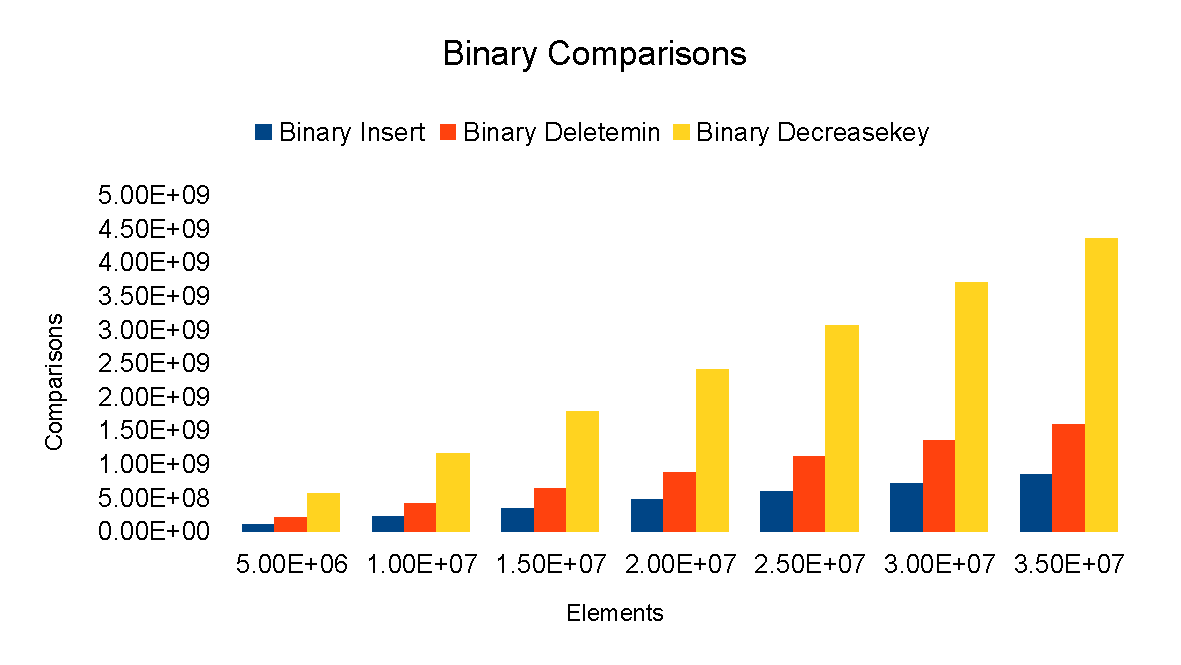
\includegraphics[width=\textwidth]{graphs/bin_comp.pdf}
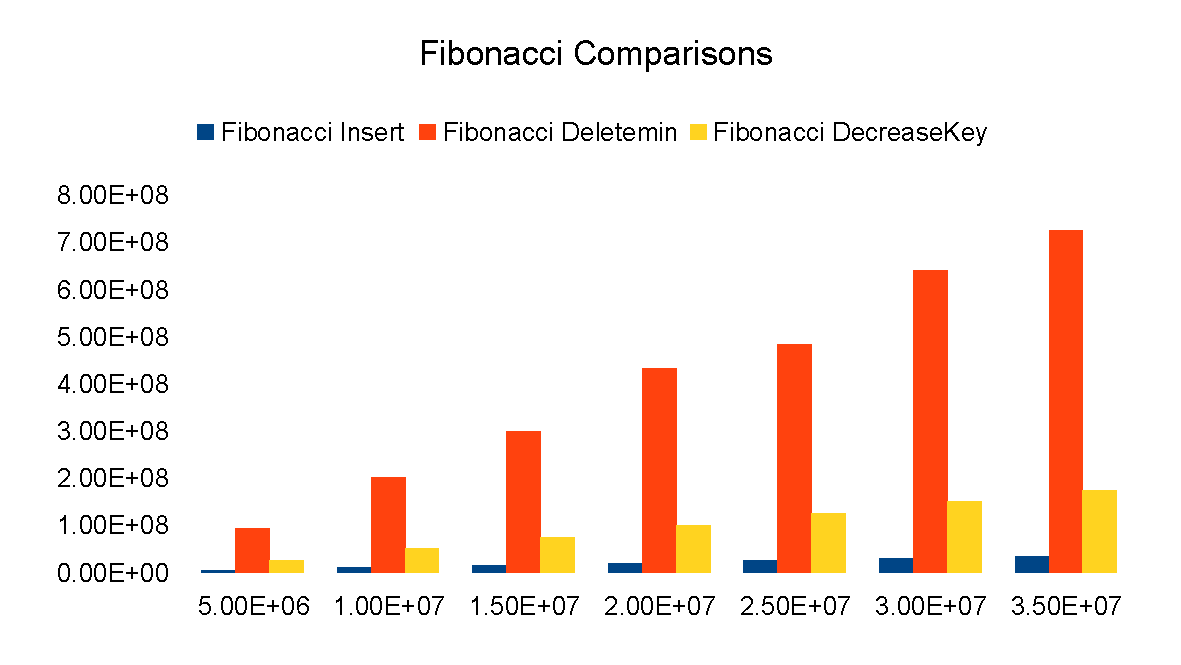
\includegraphics[width=\textwidth]{graphs/fib_comp.pdf}

We can see that the binary heap spends most comparisons in its decreasekey operation, whereas the fibonacci heap spends them in the deletemin operation because it defers fixing up the structure after insert and decreasekey operations until it needs to do so after deleting a node in the deletemin operation.

Also note the axis: even though the fibonacci heap does a lot of comparisons when doing deletemin, it is still less than what the binary heap does with the same amount of elements.

\subsection{Conclusions from the running times}
From our data, we see that our implemented data structures perform as expected from theoretical analysis, with the fibonacci heap heavily outperforming the  binary heap on inserts and decreasekey, while being somewhat slower on deletes, due to being more complex in  general.
Note that one of the reasons why the fibonacci heap performs exceedingly well on decreasekey is that the tree structures are never constructed by a deletemin, instead the entire heap is one huge list of single nodes. 


